\section{コースB: ハーフ・ポジション}
\begin{center}
\begin{tabular}{|lcl|}
\hline
この章の基礎練習 & : & 開放弦の練習\\ 
この章の修了課題 & : & 1. 「\ref{half_scale}」の音階練習を正しい音程で暗譜して演奏できる\\
               &   & 2. サン=サーンスの「亀」を正しい音程で暗譜して演奏できる\\
\hline
\end{tabular}
\end{center}
\subsection{ベーシストの左手をつくる}
\begin{flushleft}
\begin{minipage}{203pt}
\ \ \ \ 左手の練習に入る前に、左手の中指と薬指が離れないように縛ってく
ださい(図\addtocounter{figure}{1}\thefigure)。左手の形が身に付くまでは
図\thefigure のように指を縛ってから練習します。比較的開きにくい人差指
と中指の間を広げるには、図\addtocounter{figure}{1}\thefigure のように
ネックの根元に指の間を差し込むことを続けると有効です。\\
\end{minipage}
\hfill
\begin{minipage}{110pt}
\addtocounter{figure}{-1}
\begin{center}
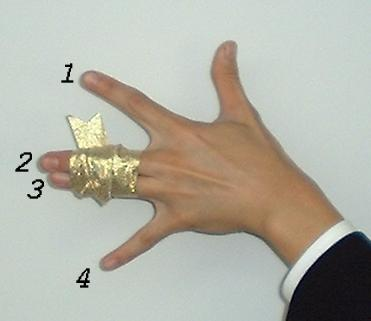
\includegraphics[height=3.6cm]{../Vol1/Pics/Position/fingering.epsi}\\
{\small 図\thefigure : 指番号と縛る指\\}
\end{center}
\end{minipage}
\hfill
\begin{minipage}{120pt}
\addtocounter{figure}{1}
\begin{center}
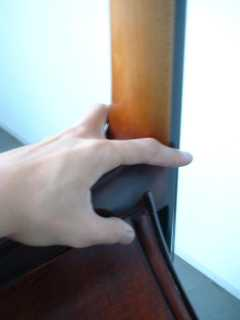
\includegraphics[height=3.6cm]{../Vol1/Pics/photo0830/open_finger.epsi}\\
{\small 図\thefigure : ネックの根元に差し込む\\}
\end{center}
\end{minipage}
\end{flushleft}
\ \ \ \ 左手の指には図\addtocounter{figure}{-1}\thefigure のように番号が付いています。音符の上
に書いてある数字に対応する指で弦を押さえます。例えば、4と書いてあった
ら小指で弦を押さえます。開放弦は0で表されます。3の指は第\ref{6th}章ま
で使いません。

\subsection{ハーフ・ポジションの位置と弦の押さえ方}
\begin{flushleft}
\begin{minipage}{160pt}
 ネック上における左手の位置のことをポジションと言います。ここ
からの章ではオーケストラでの演奏に必要なポジションを1つずつマスターし
ていきます。最初に紹介するハーフ・ポジションはネックの上端にあるポジショ
ンです(図\addtocounter{figure}{2}\thefigure 、 
\addtocounter{figure}{1}\thefigure)。親指は2の指の裏側に置きます(図\addtocounter{figure}{1}\thefigure)。
\end{minipage}
\hfill
\begin{minipage}{80pt}
\addtocounter{figure}{-2}
\begin{center}
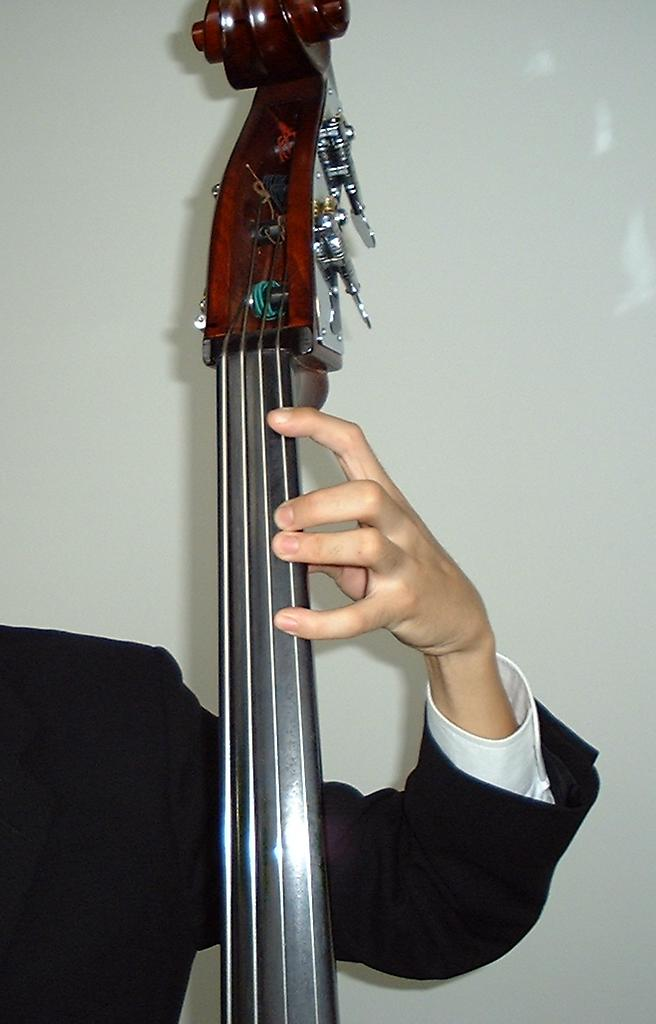
\includegraphics[height=4.3cm]{../Vol1/Pics/Position/half_1.epsi}\\
\end{center}
{\small 図\thefigure : ハーフ・ポジションの位置\\}
\end{minipage}
\hfill
\begin{minipage}{80pt}
\addtocounter{figure}{1}
\begin{center}
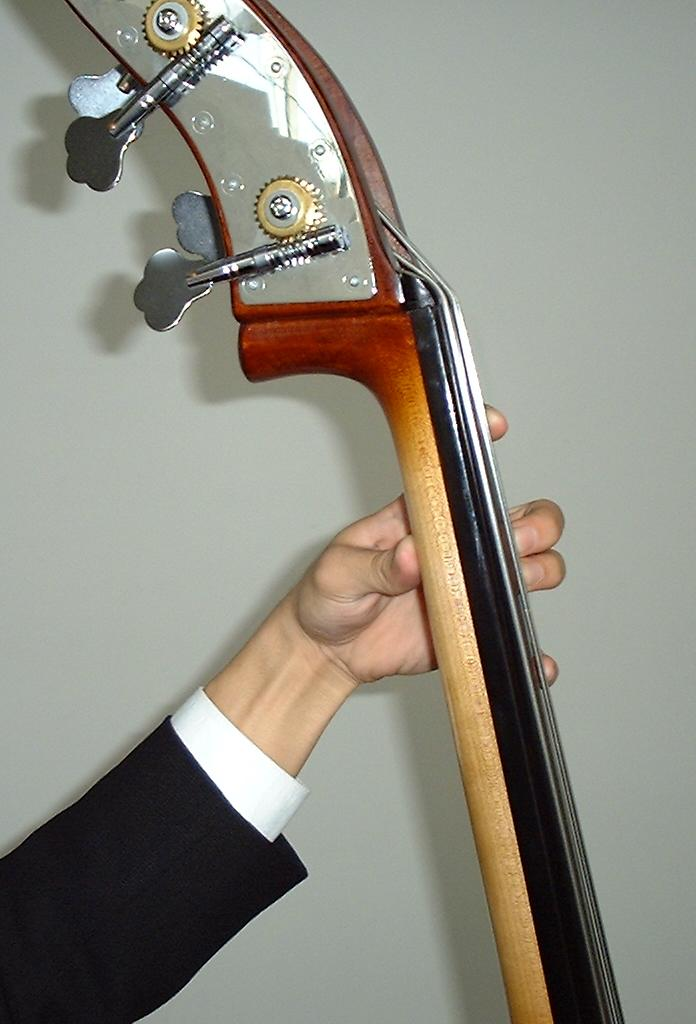
\includegraphics[height=4.3cm]{../Vol1/Pics/Position/half_3.epsi}\\
\end{center}
{\small 図\thefigure : 奏者から見たハーフ・ポジション}\\
\end{minipage}
\hfill
\begin{minipage}{85pt}
\addtocounter{figure}{1}
\begin{center}
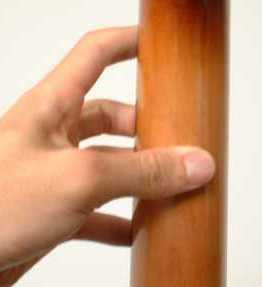
\includegraphics[height=4.3cm]{../Vol1/Pics/photo0830/left_thumb1.epsi}\\
\end{center}
{\small 図\thefigure : 左手親指の位置   }\\
\end{minipage}
\end{flushleft}
\indent 弦を押さえる際には1と2、2と4の指の間が均等に開くようにし、指の
先で押さえます(図\addtocounter{figure}{-2}\thefigure)。1の指はネックの
上側に少し傾け、指のやや側面寄りの位置で押さえます(図
\addtocounter{figure}{3}\thefigure)。 指は丸めてアーチ状にします(図
\thefigure)。図\addtocounter{figure}{1}\thefigure のようにつぶれたアー
チは正しくありません。
\begin{flushleft}
\begin{minipage}{220pt}
 また、2、4の指で押さえる場合には必ず上側の指も一緒に押さえます
(図\addtocounter{figure}{1}\thefigure)。たとえば2の指を押さえる際に
1を放してはいけません(図\addtocounter{figure}{1}\thefigure)。\\

\begin{minipage}{100pt}
\addtocounter{figure}{-3}
\begin{center}
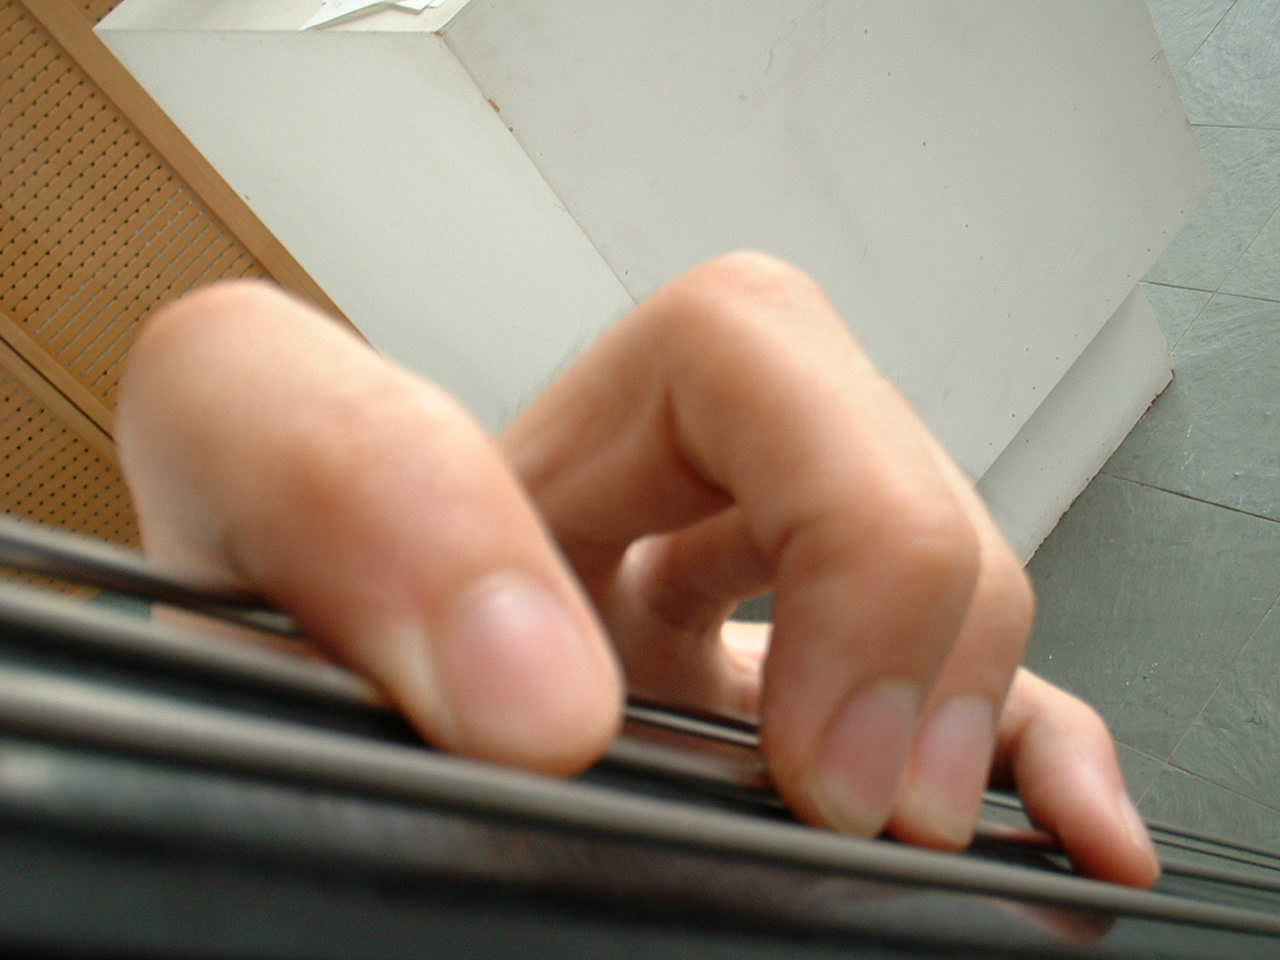
\includegraphics[height=2cm]{../Vol1/Pics/newphoto/arch1.epsi}\\
\end{center}
{\small 図\thefigure : アーチ状に丸める。1は指の側面で押さえる。\\}
\end{minipage}
\hfill
\begin{minipage}{100pt}
\addtocounter{figure}{1}
\begin{center}
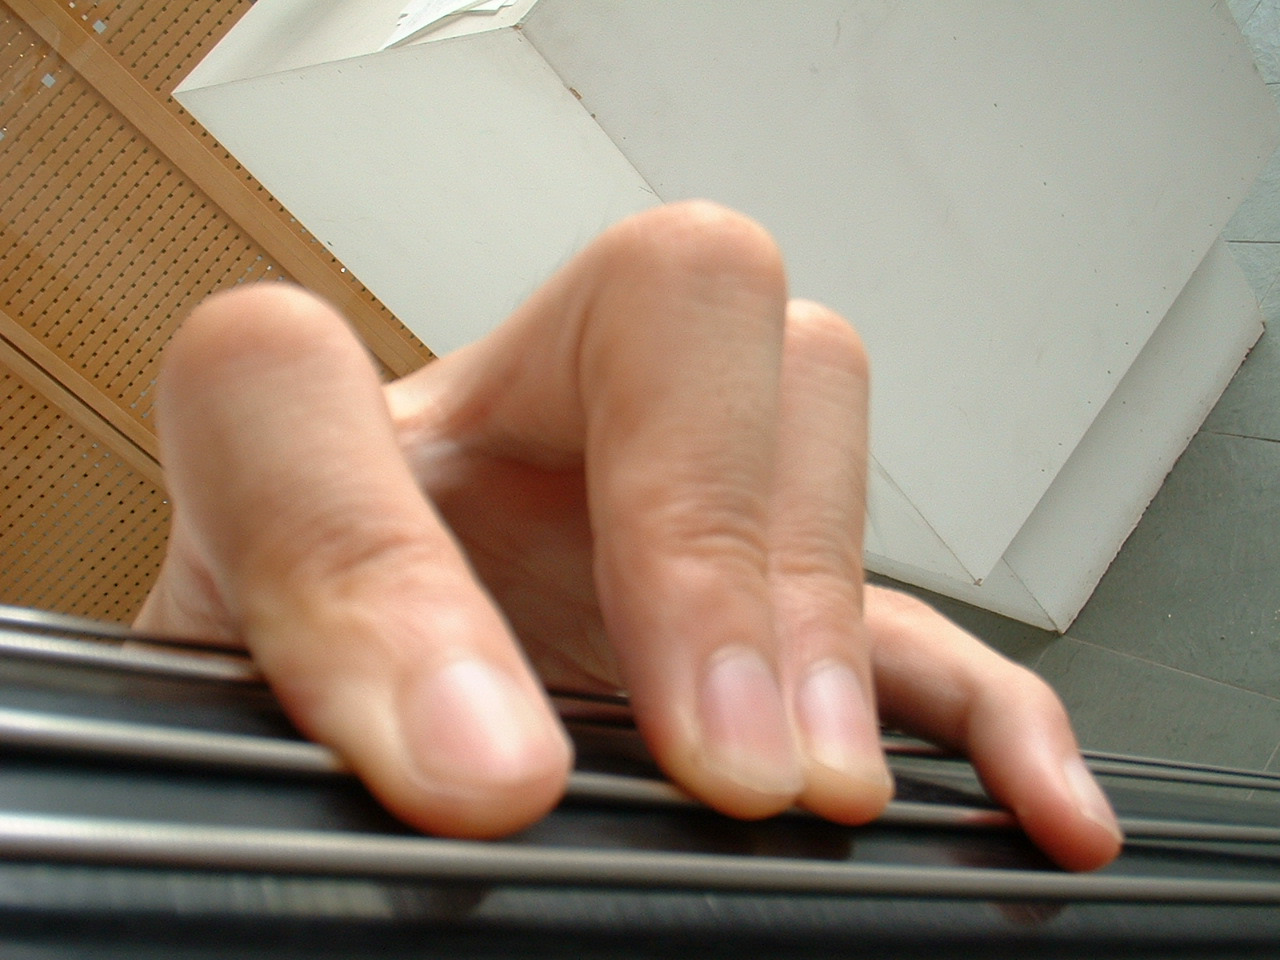
\includegraphics[height=2cm]{../Vol1/Pics/newphoto/arch2.epsi}\\
\end{center}
{\small 図\thefigure : アーチがつぶれてはダメ\\}
\end{minipage}
\end{minipage}
\hfill
\begin{minipage}{100pt}
\addtocounter{figure}{1}
\begin{center}
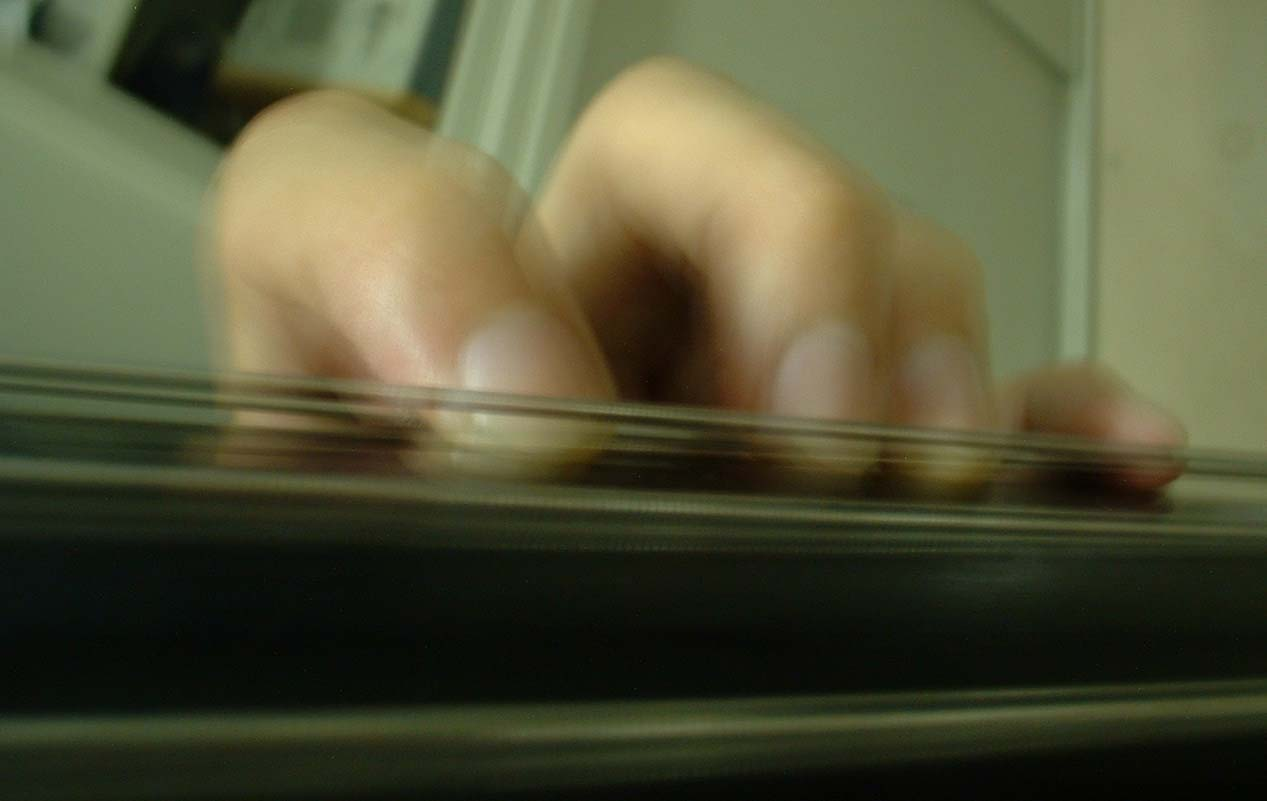
\includegraphics[width=3cm]{../Vol1/Pics/newphoto/finger1.epsi}\\
\end{center}
{\small 図\thefigure : 1の指も一緒に\\}
\end{minipage}
\hfill
\begin{minipage}{100pt}
\addtocounter{figure}{1}
\begin{center}
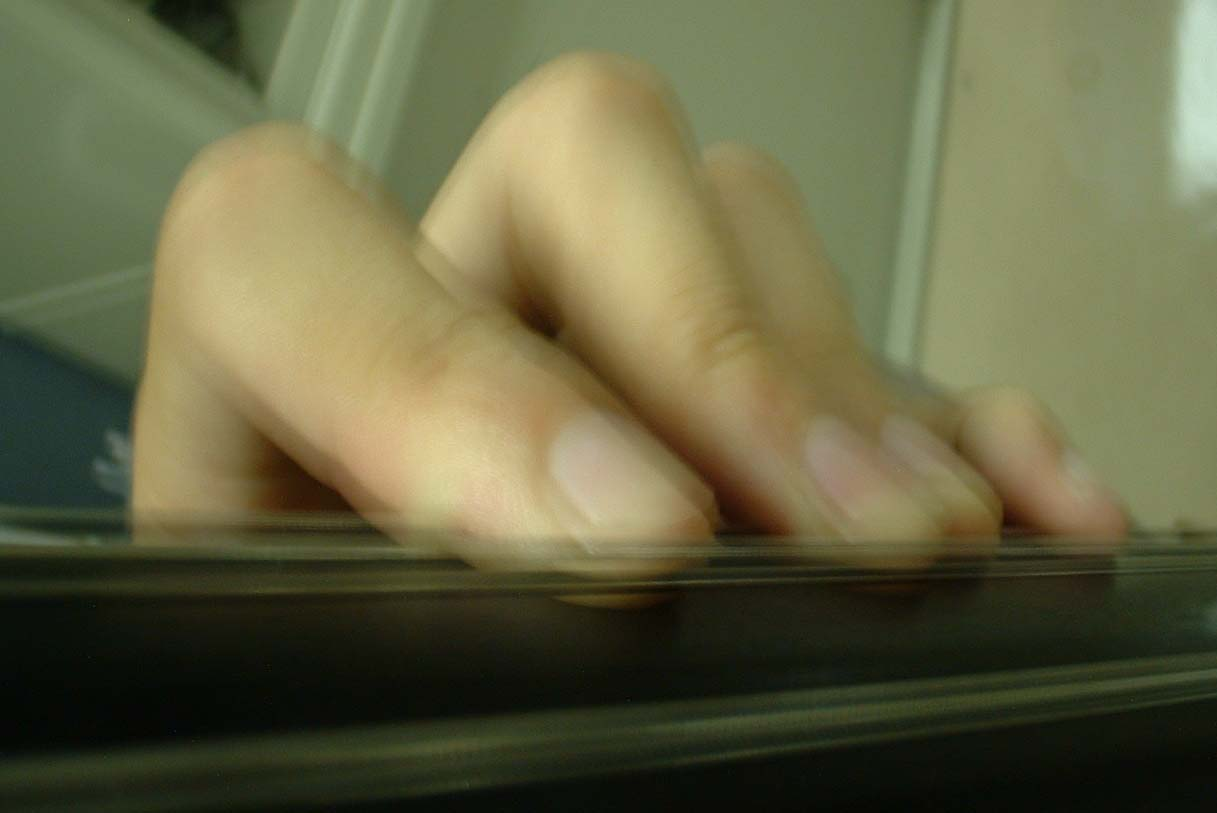
\includegraphics[width=3cm]{../Vol1/Pics/newphoto/finger2.epsi}\\
\end{center}
{\small 図\thefigure : 1を放してはダメ\\}
\end{minipage}
\end{flushleft}

\subsection{肘の位置}
\begin{flushleft}
\begin{minipage}{250pt}
 弦の押さえ方を覚えたら、次は肘の位置を習得しましょう。前腕(手首から肘まで)の角度が、ネックの上下方向と直角になる位置まで肘を上げます(図\addtocounter{figure}{1}\thefigure)。\\

\ \ \ \ 4の指は他の指と比べて押さえる力が弱いですが、このように肘を上げることで4の指の力を腕の重みで補えるようになります。
\end{minipage}
\hfill
\begin{minipage}{180pt}
\begin{center}
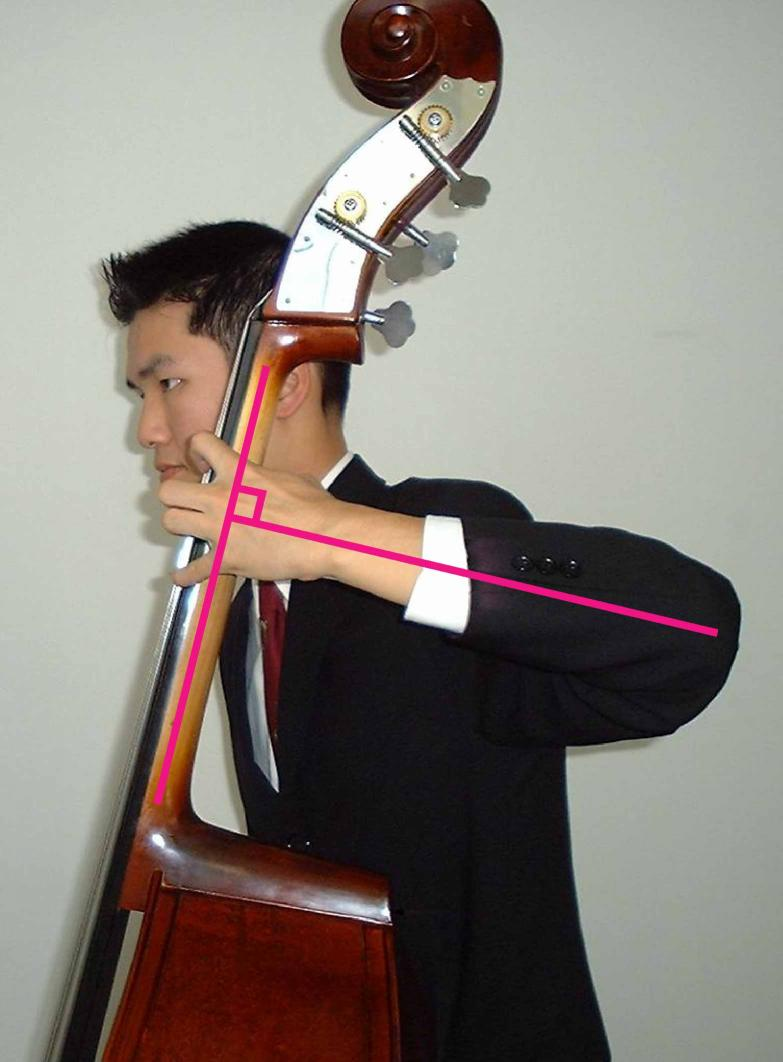
\includegraphics[height=4.5cm]{../Vol1/Pics/Shifting/orthogonal_halfsize.epsi}\\
図\thefigure : 腕とネックが直角になるのが目安\\
\end{center}
\end{minipage}
\end{flushleft}

\subsection{ハーフ・ポジションで取れる音}
ハーフ・ポジションではそれぞれの弦で以下の音を取ることができます。正し
い場所を押さえているかどうか、チューニングメーターで確認しながら弾いてみましょう。\\

\begin{music}
\nostartrule
\parindent 0pt
\setclef1{\bass}  
\startpiece
\notes\enotes
\Notes\zchar{16}{G線}\zchar{11}{\bf 1}\wh{'^G}\zchar{11}{\bf 2}\wh{!=a}\zchar{11}{\bf 4}\wh{^a}\enotes
\doublebar
\Notes\zchar{11}{\bf 1}\wh{_a}\zchar{11}{\bf 2}\wh{=a}\zchar{11}{\bf 4}\wh{_b}\enotes
\doublebar
\Notes\zchar{16}{D線}\zchar{9}{\bf 1}\wh{'^D}\zchar{9}{\bf 2}\wh{E}\zchar{9}{\bf 4}\wh{F}\enotes
\doublebar
\Notes\zchar{9}{\bf 1}\wh{'_E}\zchar{9}{\bf 2}\wh{=E}\zchar{9}{\bf 4}\wh{F}\enotes
\setdoublebar
\endpiece
\startpiece
\notes\enotes
\Notes\zchar{14}{A線}\zchar{9}{\bf 1}\wh{'^A}\zchar{9}{\bf 2}\wh{B}\zchar{9}{\bf 4}\wh{C}\enotes
\doublebar
\Notes\zchar{9}{\bf 1}\wh{'_B}\zchar{9}{\bf 2}\wh{=B}\zchar{9}{\bf 4}\wh{C}\enotes\doublebar
\Notes\zchar{14}{E線}\zchar{9}{\bf 1}\wh{F}\zchar{9}{\bf 2}\wh{^F}\zchar{9}{\bf 4}\wh{G}\enotes
\doublebar
\Notes\zchar{9}{\bf 1}\wh{F}\zchar{9}{\bf 2}\wh{_G}\zchar{9}{\bf 4}\wh{G}\enotes
\setdoublebar
\endpiece
\end{music}

\subsection{音階練習 \label{half_scale}}
\begin{music}
\nostartrule
\parindent 0pt
\setclef1{\bass}  
\generalmeter{\meterC}
\generalsignature{-1}    
\startpiece
\notes\zchar{14}{ヘ長調(F-dur)音階}\enotes
\NOtes\zchar{9}{\bf 1}\qu{F}\zchar{9}{\bf 4}\qu{G}\zchar{9}{\bf 0}\qu{'A}\zchar{9}{\bf 1}\qu{B}\enotes
\bar
\NOtes\zchar{9}{\bf 4}\qu{'C}\zchar{9}{\bf 0}\ql{D}\zchar{9}{\bf 2}\ql{E}\zchar{9}{\bf 4}\ql{F}\enotes
\bar
\NOtes\zchar{9}{\bf 4}\ql{'F}\zchar{9}{\bf 2}\ql{E}\zchar{9}{\bf 0}\ql{D}\zchar{9}{\bf 4}\qu{C}\enotes
\bar
\NOtes\zchar{9}{\bf 1}\qu{'B}\zchar{9}{\bf 0}\qu{A}\zchar{9}{\bf 4}\qu{!G}\zchar{9}{\bf 1}\qu{F}\enotes
\setdoublebar
\endpiece

\generalmeter{\meterC}
\generalsignature{-2}    
\startpiece
\notes\zchar{14}{変ロ長調(B-dur)音階}\enotes
\NOtes\zchar{9}{\bf 1}\qu{'B}\zchar{9}{\bf 4}\qu{C}\zchar{9}{\bf 0}\ql{D}\zchar{9}{\bf 1}\ql{E}\enotes
\bar
\NOtes\zchar{9}{\bf 4}\ql{'F}\zchar{9}{\bf 0}\ql{G}\zchar{10}{\bf 2}\ql{!a}\zchar{11}{\bf 4}\ql{b}\enotes
\bar
\NOtes\zchar{11}{\bf 4}\ql{b}\zchar{10}{\bf 2}\ql{a}\zchar{9}{\bf 0}\ql{'G}\zchar{9}{\bf 4}\ql{F}\enotes
\bar
\NOtes\zchar{9}{\bf 1}\ql{'E}\zchar{9}{\bf 0}\ql{D}\zchar{9}{\bf 4}\qu{C}\zchar{9}{\bf 1}\qu{B}\enotes
\setdoublebar\endpiece
\end{music}

\subsection{ハーフ・ポジションだけで弾ける名曲}
\documentclass{jarticle}
\usepackage{musixdoc}
\startmuflex\makeindex

\begin{document}

\subsubsection*{����᥵���� : �ȶʡ�ưʪ�μ����ספ��ֵ���}

\begin{music}
\nostartrule
\setclef1{\bass}
\generalsignature{-2}    
\generalmeter{\meterfrac44}
\parindent 0pt
\startbarno=3
\def\writebarno{\tenrm\the\barno\barnoadd}
\def\raisebarno{2\internote}
\def\shiftbarno{0.1\Interligne}
\systemnumbers
\startpiece\bigaccid
\notes\zchar{20}{\bf Andante maestoso}\zchar{-4}{\pp}\enotes
\NOtes\zchar{12}{\upbow}\zchar{9}{\bf 1}\hu{'B}\enotes
\notes\ibu{0}{'E}{0}\zchar{16}{\downbow}\zchar{13}{\bf 4}\qb{0}{C}\zchar{16}{\upbow}\zchar{13}{\bf 1}\qb{0}{E}\zchar{16}{\downbow}\zchar{13}{\bf 0}\qb{0}{D}\tbu{0}\zchar{16}{\upbow}\zchar{13}{\bf 4}\qb{0}{C}\enotes
\bar
\Notes\zchar{12}{\downbow}\zchar{9}{\bf 4}\ql{'F}\zchar{12}{\upbow}\zchar{9}{\bf 4}\ql{F}\enotes
\notes\ibl{0}{'E}{-2}\zchar{12}{\downbow}\zchar{9}{\bf 4}\qb{0}{F}\zchar{12}{\upbow}\zchar{9}{\bf 0}\qb{0}{G}\zchar{12}{\downbow}\zchar{9}{\bf 0}\qb{0}{D}\tbl{0}\zchar{12}{\upbow}\zchar{9}{\bf 1}\qb{0}{E}\enotes
\bar
\Notes\zchar{12}{\downbow}\zchar{9}{\bf 4}\qu{'C}\zchar{12}{\upbow}\zchar{9}{\bf 4}\qu{C}\enotes
\notes\ibl{0}{'D}{0}\zchar{12}{\downbow}\zchar{9}{\bf 4}\qb{0}{C}\zchar{12}{\upbow}\zchar{9}{\bf 1}\qb{0}{E}\zchar{12}{\downbow}\zchar{9}{\bf 0}\qb{0}{D}\tbl{0}\zchar{12}{\upbow}\zchar{9}{\bf 4}\qb{0}{C}\enotes
\bar
\notes\ibl{0}{'D}{2}\zchar{12}{\downbow}\zchar{9}{\bf 1}\qb{0}{B}\zchar{14}{\upbow}\zchar{11}{\bf 4}\qb{0}{!b}\zchar{13}{\downbow}\zchar{10}{\bf 2}\qb{0}{a}\tbl{0}\zchar{12}{\upbow}\zchar{9}{\bf 0}\qb{0}{'G}\enotes
\notes\ibl{0}{'F}{-3}\zchar{12}{\downbow}\zchar{9}{\bf 4}\qb{0}{F}\zchar{12}{\upbow}\zchar{9}{\bf 1}\qb{0}{E}\zchar{12}{\downbow}\zchar{9}{\bf 0}\qb{0}{D}\tbl{0}\zchar{12}{\upbow}\zchar{9}{\bf 4}\qb{0}{C}\enotes
\bar
\NOtes\zchar{12}{\downbow}\zchar{9}{\bf 1}\hu{'B}\enotes
\notes\ibu{0}{'E}{0}\zchar{16}{\downbow}\zchar{13}{\bf 4}\qb{0}{C}\zchar{16}{\upbow}\zchar{13}{\bf 1}\qb{0}{E}\zchar{16}{\downbow}\zchar{13}{\bf 0}\qb{0}{D}\tbu{0}\zchar{16}{\upbow}\zchar{13}{\bf 4}\qb{0}{C}\enotes
\bar
\Notes\zchar{12}{\downbow}\zchar{9}{\bf 4}\ql{'F}\zchar{12}{\upbow}\zchar{9}{\bf 4}\ql{F}\enotes
\notes\ibl{0}{'E}{-2}\zchar{12}{\downbow}\zchar{9}{\bf 4}\qb{0}{F}\zchar{12}{\upbow}\zchar{9}{\bf 0}\qb{0}{G}\zchar{12}{\downbow}\zchar{9}{\bf 0}\qb{0}{D}\tbl{0}\zchar{12}{\upbow}\zchar{9}{\bf 1}\qb{0}{E}\enotes
\bar
\Notes\zchar{12}{\downbow}\zchar{9}{\bf 4}\qu{'C}\zchar{12}{\upbow}\zchar{9}{\bf 4}\qu{C}\enotes
\notes\ibl{0}{'D}{0}\zchar{12}{\downbow}\zchar{9}{\bf 4}\qb{0}{C}\zchar{12}{\upbow}\zchar{9}{\bf 1}\qb{0}{E}\zchar{12}{\downbow}\zchar{9}{\bf 0}\qb{0}{D}\tbl{0}\zchar{12}{\upbow}\zchar{9}{\bf 4}\qb{0}{C}\enotes
\bar
\notes\ibl{0}{'C}{1}\zchar{12}{\downbow}\zchar{9}{\bf 1}\qb{0}{B}\zchar{12}{\upbow}\zchar{9}{\bf 4}\qb{0}{F}\zchar{12}{\downbow}\zchar{9}{\bf 4}\qb{0}{C}\tbl{0}\zchar{12}{\upbow}\zchar{9}{\bf 0}\qb{0}{D}\enotes
\Notes\zchar{12}{\downbow}\zchar{9}{\bf 1}\qu{'B}\qp\enotes
\mulooseness=0
\setdoublebar\endpiece
\end{music}

\endmuflex
\end{document}

\documentclass{jarticle}
\usepackage{musixdoc}
\startmuflex\makeindex

\begin{document}

\subsubsection*{���祹������������ : �������5�� ��2�ھ���Ƭ}

\begin{music}
\nostartrule
\setclef1{\bass}  
\generalmeter{\meterfrac34}
\parindent 0pt
\def\writebarno{\tenrm\the\barno\barnoadd}
\def\raisebarno{2\internote}
\def\shiftbarno{0.1\Interligne}
\systemnumbers
\startpiece\bigaccid
\notes\zchar{17}{\bf Allegretto}\enotes
\Notes\zchar{-5}{\ff}\zchar{10}\downbow\zchar{7}{\bf 2}\ql{'E}\qp\zchar{9}\upbow\zchar{6}{\bf 0}\ql{D}\enotes
\bar
\Notes\zchar{12}\downbow\zchar{9}{\bf 4}\qu{'C}\zchar{12}\upbow\zchar{9}{\bf 0}\ql{D}\zchar{12}\downbow\zchar{9}{\bf 2}\qu{B}\enotes
\bar
\Notes\zchar{12}\upbow\zchar{9}{\bf 4}\qu{'C}\enotes
\notes\ibu{0}{E}{3}\zchar{10}\downbow\zchar{7}{\bf 0}\qb{0}{E}\tbu{0}\zchar{10}\upbow\zchar{7}{\bf 1}\qb{0}{F}\enotes
\Notes\zchar{10}\downbow\zchar{7}{\bf 4}\qu{G}\enotes
\bar
\Notes\zchar{11}\upbow\zchar{8}{\bf 2}\qu{'B}\enotes
\notes\ibu{0}{E}{3}\zchar{9}\downbow\zchar{6}{\bf 0}\qb{0}{E}\tbu{0}\zchar{9}\upbow\zchar{6}{\bf 1}\qb{0}{F}\enotes
\Notes\zchar{9}\downbow\zchar{7}{\bf 4}\qu{G}\enotes
\bar
\notes\ibu{0}{'A}{0}\zchar{9}\downbow\zchar{-4}{\bf 0}\qb{0}{A}\tbu{0}\zchar{9}\upbow\zchar{-4}{\bf 0}\qb{0}{A}\ibu{0}{A}{0}\zchar{-4}{\bf 0}\qb{0}{A}\tbu{0}\zchar{-4}{\bf 0}\qb{0}{A}\ibu{0}{A}{3}\zchar{-4}{\bf 0}\qb{0}{A}\tbu{0}\zchar{-3}{\bf 2}\qb{0}{B}\enotes
\bar
\notes\ibu{0}{'C}{3}\zchar{11}\downbow\zchar{-2}{\bf 4}\qb{0}{C}\tbu{0}\zchar{11}\upbow\zchar{-2}{\bf 0}\qb{0}{D}\ibl{0}{E}{3}\zchar{9}{\bf 2}\qb{0}{E}\tbl{0}\zchar{9}{\bf 4}\qb{0}{F}\ibl{0}{G}{3}\zchar{9}{\bf 0}\qb{0}{G}\tbl{0}\zchar{9}{\bf 2}\qb{0}{!a}\enotes
\bar
\Notes\zchar{14}\downbow\zchar{11}{\bf 4}\ql{_b}\enotes
\notes\ibl{0}{a}{3}\zchar{14}\upbow\zchar{11}{\bf 2}\qb{0}{a}\tbl{0}\zchar{14}\downbow\zchar{11}{\bf 4}\qb{0}{b}\ibl{0}{a}{3}\zchar{14}\upbow\zchar{11}{\bf 2}\qb{0}{a}\tbl{0}\zchar{14}\downbow\zchar{11}{\bf 4}\qb{0}{b}\enotes
\bar
\Notes\zchar{13}\upbow\zchar{10}{\bf 0}\ql{'G}\enotes
\notes\ibl{0}{'G}{3}\zchar{13}\downbow\zchar{10}{\bf 0}\qb{0}{G}\tbl{0}\zchar{13}\upbow\zchar{10}{\bf 2}\qb{0}{!a}\ibl{0}{'G}{3}\zchar{13}\downbow\zchar{10}{\bf 0}\qb{0}{G}\tbl{0}\zchar{13}\upbow\zchar{10}{\bf 2}\qb{0}{!a}\enotes
\bar
\Notes\zchar{11}\downbow\zchar{8}{\bf 4}\ql{'F}\zchar{12}\upbow\zchar{9}{\bf 0}\ql{G}\zchar{11}\downbow\zchar{8}{\bf 2}\ql{E}\enotes
\bar
\Notes\zchar{11}\upbow\zchar{8}{\bf 4}\ql{'F}\zchar{9}\downbow\zchar{6}{\bf 0}\ql{D}\zchar{10}\upbow\zchar{7}{\bf 2}\ql{E}\enotes
\bar
\Notes\zchar{9}\downbow\zchar{-2}{\bf 4}\qu{'C}\zchar{9}\upbow\zchar{-4}{\bf 4}\qu{!G}\qp\enotes
\bar
\Notes\zchar{9}\downbow\zchar{-3}{\bf 1}\qu{_!'B}\zchar{9}\upbow\zchar{-6}{\bf 1}\qu{!F}\qp\enotes
\bar
\Notes\zchar{9}\downbow\zchar{-4}{\bf 0}\qu{'A}\zchar{9}\upbow\zchar{-7}{\bf 0}\qu{!E}\qp\enotes
\mulooseness=0
\setdoublebar\endpiece
\end{music}

\endmuflex
\end{document}

\documentclass{jarticle}
\usepackage{musixdoc}
\startmuflex\makeindex

\begin{document}

\subsubsection*{�١��ȡ�������: �������3�� �ѥ�ĹĴ�ֱ�ͺ�� ��4�ھϤ��}
\begin{music}
\nostartrule
\setclef1{\bass}  
\generalsignature{-3}    
\generalmeter{\meterfrac34}
\parindent 0pt
\startbarno=12
\def\writebarno{\tenrm\the\barno\barnoadd}
\def\raisebarno{2\internote}
\def\shiftbarno{0.1\Interligne}
\systemnumbers
\startpiece\bigaccid
\notes\zchar{17}{\bf Allegro molto (\metron{\hu}{76})}\enotes
\Notes\cl{'E}\ds\qp\enotes
\bar
\Notes\cl{b}\ds\qp\enotes
\bar
\Notes\cu{'B}\ds\qp\enotes
\bar
\Notes\cl{'E}\ds\qp\enotes
\bar
\Notes\cl{'E}\ds\cl{D}\ds\enotes
\bar
\Notes\ql{'E}\ds\cl{=E}\enotes
\bar
\Notes\ibu{0}{'F}{-1}\qb{0}{FD_E}\tbu{0}\qb{0}{=A}\enotes
\bar
\Notes\qu{'B}\enotes
\bar
\Notes\ql{'E}\qp\enotes
\bar
\Notes\ql{b}\qp\enotes
\bar
\Notes\qu{'B}\qp\enotes
\bar
\Notes\ql{'E}\qp\enotes
\bar
\Notes\cl{'E}\ds\cl{D}\ds\enotes
\bar
\Notes\ql{'E}\ds\cl{=E}\enotes
\bar
\Notes\ibu{0}{'F}{-1}\qb{0}{FD_E}\tbu{0}\qb{0}{=A}\enotes
\bar
\Notes\qu{'B}\enotes
\bar
\notes\zchar{8}{\Large\bf \ 3}\PAuse\pause\enotes
\bar
\Notes\qp\ds\cl{a}\enotes
\bar
\Notes\cl{'G}\ds\qp\enotes
\bar
\Notes\cl{a}\ds\qp\enotes
\bar
\Notes\cl{b}\ds\cl{b}\ds\enotes
\bar
\Notes\cl{'E}\ds\qp\enotes
\bar
\Notes\ibu{0}{'B}{0}\qb{0}{BB}\tbu{0}\qb{0}{B}\ds\enotes
\bar
\notes\zchar{8}{\Large\bf \ 1}\enotes
\Notes\pause\enotes
\bar
\Notes\qup{'B}\ds\enotes
\bar
\Notes\qp\ds\cl{a}\enotes
\bar
\Notes\cl{'G}\ds\qp\enotes
\bar
\Notes\cl{a}\ds\qp\enotes
\bar
\Notes\cl{b}\ds\cl{b}\ds\enotes
\bar
\Notes\cl{'E}\ds\qp\enotes
\setdoublebar
\endpiece
\end{music}

\endmuflex
\end{document}

